
\documentclass[8pt,mathserif]{beamer}
\usepackage{etex}
\usetheme{Warsaw}
\usecolortheme{whale}
\usepackage{times}  % fonts are up to you
\usepackage{graphicx}
\usepackage{verbatim}
\usepackage{amsmath}
\usepackage{color}
\usepackage{listings}
\usepackage{lmodern}
\usepackage{multicol}
\usepackage{epsfig}
\usepackage[T1]{fontenc}
\usepackage{lib/qcircuit}
% quantum macros

\def\01{\{0,1\}}
\def\eps{\epsilon}
\newcommand{\half}{{\frac{1}{2}}}
\newcommand{\set}[1]{{\left\{#1\right\}}}
\newcommand{\ksubsets}{{n \choose k}}
\newcommand{\jsubsets}{{n \choose j}}
\newcommand{\Prob}{{\mathbf{Pr}}}
\newcommand{\tinyspace}{\mspace{1mu}}
\newcommand{\microspace}{\mspace{0.5mu}}
\newcommand{\op}[1]{\operatorname{#1}}

\newcommand{\norm}[1]{\left\lVert\tinyspace#1\tinyspace\right\rVert}
\newcommand{\snorm}[1]{\lVert\tinyspace#1\tinyspace\rVert}
\newcommand{\abs}[1]{\left\lvert\tinyspace #1 \tinyspace\right\rvert}
\newcommand{\ceil}[1]{\left\lceil #1 \right\rceil}
\newcommand{\floor}[1]{\left\lfloor #1 \right\rfloor}
\def\iso{\cong}
\newcommand{\defeq}{\stackrel{\smash{\text{\tiny def}}}{=}}
\newcommand{\tr}{\operatorname{tr}}
\newcommand{\rank}{\operatorname{rank}}
\renewcommand{\det}{\operatorname{Det}}
\newcommand{\im}{\operatorname{Im}}
\renewcommand{\t}{{\scriptscriptstyle\mathsf{T}}}
\newcommand{\ip}[2]{\left\langle #1 , #2\right\rangle}
\newcommand{\ipp}[1]{\left\langle #1 \right\rangle}
\newcommand{\sip}[2]{\langle #1 | #2\rangle}

\def\({\left(}
\def\){\right)}
\def\I{\mathsf{id}}

\newcommand{\fid}{\operatorname{F}}
\newcommand{\setft}[1]{\mathrm{#1}}
\newcommand{\lin}[1]{\setft{L}\left(#1\right)}
\newcommand{\density}[1]{\setft{Dens}\left(#1\right)}
\newcommand{\unitary}[1]{\setft{U}\left(#1\right)}
\newcommand{\trans}[1]{\setft{T}\left(#1\right)}
\newcommand{\herm}[1]{\setft{Herm}\left(#1\right)}
\newcommand{\pos}[1]{\setft{Pos}\left(#1\right)}
\newcommand{\pd}[1]{\setft{Pd}\left(#1\right)}
\newcommand{\sphere}[1]{\mathcal{S}\!\left(#1\right)}
\newcommand{\opset}[3]{\setft{#1}_{#2}\!\left(#3\right)}
\newcommand{\ot}{\otimes}

\def\complex{\mathbb{C}}
\def\real{\mathbb{R}}
\def\natural{\mathbb{N}}
\def\integer{\mathbb{Z}}

\def\<{\langle}
\def\>{\rangle}
\def \lket {\left|}
\def \rket {\right\rangle}
\def \lbra {\left\langle}
\def \rbra {\right|}
\newcommand{\ket}[1]{\lket\microspace #1 \microspace\rket}
\newcommand{\bra}[1]{\lbra\microspace #1 \microspace\rbra}
\newcommand{\ketbra}[1]{\lket\microspace #1 \rangle \langle #1 \microspace\rbra}


\def\X{\mathcal{X}}
\def\Y{\mathcal{Y}}
\def\Z{\mathcal{Z}}
\def\W{\mathcal{W}}
\def\A{\mathcal{A}}
\def\B{\mathcal{B}}
\def\V{\mathcal{V}}
\def\U{\mathcal{U}}
\def\C{\mathcal{C}}
\def\D{\mathcal{D}}
\def\H{\mathcal{H}}
\def\E{\mathcal{E}}
\def\F{\mathcal{F}}
\def\M{\mathcal{M}}
\def\R{\mathcal{R}}
\def\P{\mathcal{P}}
\def\Q{\mathcal{Q}}
\def\S{\mathcal{S}}
\def\T{\mathcal{T}}
\def\K{\mathcal{K}}
\def\yes{\text{yes}}
\def\no{\text{no}}
\def\onevec{\vec{\mathbf{1}}}

\newcommand{\trnorm}[1]{\norm{#1}_{\tr}}
\newcommand{\trnormb}[1]{{\big\| #1 \big\|}_{\rm tr}}
\newcommand{\trdist}[1]{ \left | #1 \right |_{\rm tr}}
\newcommand{\uniform}[1]{\mathcal{U}_{#1}}

\def\defeq{\stackrel{\small \textrm{def}}{=}}

%Zach's note: I'm unable to compile with this package.
%   It seems like an issue with xstring
%\usepackage[style=numeric-comp]{biblatex}

%\usepackage[usenames,dvipnames]{xcolor} % for colored text
\usepackage[normalem]{ulem} % for strikethrough text



\def\BibTeX{{\rm B\kern-.05em{\sc i\kern-.025em b}\kern-.08em
    T\kern-.1667em\lower.7ex\hbox{E}\kern-.125emX}}

\newcommand*{\Scale}[2][4]{\scalebox{#1}{$#2$}}%
\newcommand{\itembase}{\setlength{\itemsep}{0pt}}
\newcommand{\eg}{{\it e.g., }}
\newcommand{\ie}{{\it i.e., }}

% All the pretty colors go here
\definecolor{myGreen}{rgb}{0,1,0}
\definecolor{myRed}{rgb}{1,0,0}
\newcommand{\clb}{\color{blue}}
\newcommand{\clr}{\color{myRed}}
\newcommand{\clg}{\color{myGreen}}
\newcommand{\clbl}{\color{black}}

% Making Qcircuit more concise
\newcommand{\uLbl}[1]{\ustick{\textit{#1}}}
\newcommand{\dblLine}{\ar@{.}[]+<0em,0em>;[d]+<0em,0em>}
\newcommand{\lzyLine}{\qw\dblLine}
\newcommand{\lzyLbl}[1]{\uLbl{#1}\qw\dblLine}

%\usepackage{bibentry}
\setbeamercolor{background canvas}{bg=gray}

\setbeamertemplate{footline}[page number]{}

%\addbibresource{TMI_bib.bib}
%\bibliography{TMIbib.bib}

\newenvironment<>{varblock}[2][.9\textwidth]{%
  \setlength{\textwidth}{#1}
  \begin{actionenv}#3%
    \def\insertblocktitle{#2}%
    \par%
    \usebeamertemplate{block begin}}
  {\par%
    \usebeamertemplate{block end}%
  \end{actionenv}}

\makeatletter
\pgfdeclareverticalshading[black,bg]{bmb@shadow}{200cm}{%
  color(0bp)=(black!25); color(4bp)=(black!50!bg); color(8bp)=(black!50!bg)}
\pgfdeclareradialshading[black,bg]{bmb@shadowball}{\pgfpointorigin}{%
  color(0bp)=(black!50!bg); color(4bp)=(black!25)}
\pgfdeclareradialshading[black,bg]{bmb@shadowballlarge}{\pgfpointorigin}{%
  color(0bp)=(black!50!bg); color(4bp)=(black!50!bg); color(8bp)=(black!25)}

\def\insertsectionnavigation#1{%
  \hbox to #1{\vbox{{\usebeamerfont{section in head/foot}%
     \usebeamercolor[fg]{section in head/foot}%
     \def\slideentry##1##2##3##4##5##6{}%
     \def\sectionentry##1##2##3##4##5{%
       \ifnum##5=\c@part%
       \def\insertsectionhead{##2\hskip1em}%
       \def\insertsectionheadnumber{##1}%
       \def\insertpartheadnumber{##5}%
         \hyperlink{Navigation##3}{%
             \ifnum\c@section=##1%
               {\usebeamertemplate{section in head/foot}}%
             \else%
               {\usebeamertemplate{section in head/foot shaded}}%
             \fi%
         }\par
       \fi}%
       \parbox[c][0cm][c]{.5\paperwidth}{%
       \begin{multicols}{2}
       \dohead
       \end{multicols}}\space}
     }%
  \hfil}%
}

\def\insertsubsectionnavigation#1{%
  \hbox to #1{%
    \vbox{{%
      \usebeamerfont{subsection in head/foot}\usebeamercolor[fg]{subsection in head/foot}%
      \vskip0.5625ex%
      \beamer@currentsubsection=0%
      \def\sectionentry##1##2##3##4##5{}%
      \def\slideentry##1##2##3##4##5##6{\ifnum##6=\c@part\ifnum##1=\c@section%
        \ifnum##2>\beamer@currentsubsection%
        \beamer@currentsubsection=##2%
        \def\insertsubsectionhead{##5}%
        \def\insertsectionheadnumber{##1}%
        \def\insertsubsectionheadnumber{##2}%
        \def\insertpartheadnumber{##6}%
        \beamer@link(##4){%
              \ifnum\c@subsection=##2%
                {\usebeamertemplate{subsection in head/foot}}%
              \else%
                {\usebeamertemplate{subsection in head/foot shaded}}%
              \fi\hfill}\par
        \fi\fi\fi}%
       \hspace*{0.5em}\parbox[c][0cm][c]{\dimexpr.5\paperwidth-1em\relax}{%
       \begin{multicols}{2}
       \dohead\vskip0.5625ex\end{multicols}
       }\space
   }\hfil
}}}

\setbeamertemplate{navigation symbols}{}
%\setbeamertemplate{blocks}[rounded][shadow=false]
%\setbeamertemplate{title page}[default][colsep=-4bp,rounded=true]
\setbeamertemplate{frametitle}[default][colsep=-4bp,rounded=false,shadow=false]

\setbeamertemplate{headline}
{%
  \leavevmode\@tempdimb=2.4375ex%
  \ifnum\beamer@subsectionmax<\beamer@sectionmax%
    \multiply\@tempdimb by\beamer@sectionmax%
  \else%
    \multiply\@tempdimb by\beamer@subsectionmax%
  \fi%
  \ifdim\@tempdimb>0pt%
    \advance\@tempdimb by 1.125ex%
    \begin{beamercolorbox}[wd=.5\paperwidth,ht=0.5\@tempdimb,dp=2ex]{section in head/foot}%
      \vbox to0.5\@tempdimb{\vfill\insertsectionnavigation{.5\paperwidth}\vfill}%
    \end{beamercolorbox}%
    \begin{beamercolorbox}[wd=.5\paperwidth,ht=0.5\@tempdimb,dp=2ex]{subsection in head/foot}%
      \vbox to0.5\@tempdimb{\vfill\insertsubsectionnavigation{.5\paperwidth}\vfill}%
    \end{beamercolorbox}%
  \fi%
}
\makeatother

\def\bra#1{\mathinner{\langle{#1}|}}
\def\ket#1{\mathinner{|{#1}\rangle}}
\newcommand{\braket}[2]{\langle #1|#2\rangle}
\def\Bra#1{\left<#1\right|}
\def\Ket#1{\left|#1\right>}

% for themes, etc.
%\mode<presentation>
%{ \usetheme{boxes} }


%\usepackage{beamerposter}

% these will be used later in the title page
\title{\bf{Cluster-State Quantum Computing}}
\author{Mayra Amezcua, Dileep V. Reddy, Zach Schmidt}
\date{\today}


% note: do NOT include a \maketitle line; also note that this title
% material goes BEFORE the \begin{document}

% have this if you'd like a recurring outline
%\AtBeginSection[]  % "Beamer, do the following at the start of every section"
%{
%\begin{frame}<beamer> 
%\frametitle{Outline} % make a frame titled "Outline"
%\tableofcontents[currentsection]  % show TOC and highlight current section
%\end{frame}
%}
\newcommand\Fontvi{\fontsize{7}{7.2}\selectfont}

\begin{document}



\usebackgroundtemplate{
\includegraphics[width=\paperwidth]{figures/fio_bg1.png}}
\begin{frame}
\begin{center}
Course Project, Spring 2016
\maketitle

{\bf CIS410/510 Introduction to Quantum Information Theory}\\
Lecturer: Prof. Xiaodi Wu\\
Computer and Information Science, University of Oregon
\end{center}
\end{frame}

\begin{frame}
{Table of Contents (optional frame. Can delete.)}
\begin{multicols}{2}
\tableofcontents
\end{multicols}
\end{frame}

\begin{frame}{template frame (delete me)}

  \begin{block}{test block}
    some text
  \end{block}

  \begin{varblock}[4cm]{test varblock}
    Variable block (here 4cm)
  \end{varblock}

  \begin{columns}

    \begin{column}{.5\linewidth}
      \begin{alertblock}{test alert}
        some alert
      \end{alertblock}
    \end{column}

    \begin{column}{.5\linewidth}
      \begin{exampleblock}{test example}
        some example citation \footnotemark
      \end{exampleblock}
    \end{column}\footnotetext[1]{Auth, DV, 123, 2001.}

  \end{columns}

\end{frame}


\section{Motivation}
\begin{frame}
\begin{gather*}
 \Qcircuit @C=1em @R=1.2em {
   & \gate{A} & \multigate{1}{C} & \qw & \gate{E} & \multigate{2}{G} & \multigate{1}{J} & \qw \\
   & \gate{B} & \ghost{C} & \gate{D}  & \multigate{1}{F} & \ghost{G} & \ghost{J} & \qw \\
   & \qw & \qw & \qw & \ghost{F} & \ghost{G} & \gate{K} & \qw \\
 }\\
 {\footnotesize \text{Arbitrary quantum circuit involving unitary operations on 3 qubits.}}%
 \end{gather*}
  One-way quantum computing, measurement based quantum computing \\
  As opposed to circuit based quantum computing
\end{frame}

\subsection{Gates through teleportation}
\begin{frame}
  Basic teleporation
\end{frame}

\section{Cluster states (CS)}

\subsection{Definition}
\begin{frame}

\end{frame}


\subsection{Representations}
\begin{frame}

    \begin{columns}

      \begin{column}{.5\linewidth}
    \begin{figure}[thb]
  \centering
  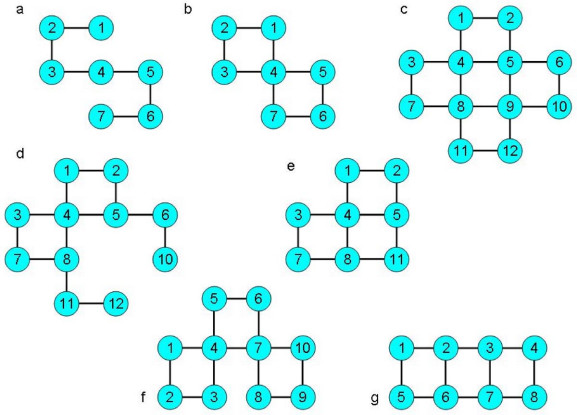
\includegraphics[width=0.9\linewidth]{figures/2d_clusters_rep.jpg}
  \label{I2dclustersfig}
  \caption{Figure showing representative 2-D cluster shapes. The vertices are qubits with integer indices, and the edges indicate entanglement connectivity between select neighbors.}
\end{figure}
        
    \end{column}

      \begin{column}{.5\linewidth}
        Blah
    \end{column}

  \end{columns}



\end{frame}


\subsection{Properties}
\begin{frame}
  
\end{frame}


\section{Universal computation through CS}

\subsection{Linear wire}
\begin{frame}
\begin{gather*}
  \Qcircuit @C=1em @R=1em{
    &\ket{\psi}_0&&&\\
    &\cluster{0}&\cluster{1}&\cluster{2}\qw&\cluster{3}\qw
    \gategroup{1}{2}{2}{3}{1.5em}{--}
}\\
{\footnotesize \text{Gate $C_z^{(0,1)}$, followed by measurements $M_X^{(0)}$, $M_X^{(1)}$, \& $M_X^{(2)}$.}}%
\end{gather*}
\end{frame}

\subsection{Arbitrary single qubit operations}
\begin{frame}
  Callback to teleportation discussion
  
\begin{gather*}
\Qcircuit @C=1em @R=1em{
&\lstick{\ket{+}_1} &\ctrl{1} & \gate{HZ_{\alpha1}} & \meter & \cw & \cw \\
&\lstick{\ket{+}_2} & \gate{CZ} & \qw & \qw & \ctrl{1} & \gate{HZ_{\pm\alpha2}} \cwx  & \meter \\
&\lstick{\ket{+}_3} & \qw & \qw & \qw & \gate{CZ} & \qw & \qw \gategroup{1}{5}{2}{3}{0.8em}{--} \gategroup{2}{6}{3}{8}{1.2em}{--}
}
\end{gather*}

\end{frame}


\subsection{Two qubit operations}
\begin{frame}
\newcommand{\bertLine}{\ar@{-}[]+<0em,-2.3em>;[d]+<0em,2.3em>}
\begin{gather*}
  \Qcircuit @C=1em @R=1em{
    \ket{\phi_A}&\cluster{\Scale[0.8] A}&\cluster{1}&\qw&\cluster{2}\bertLine\qw&\qw&\cluster{3}\qw\\
    \ket{\phi_B}&\cluster{\Scale[0.8] B}&\cluster{5}&\qw&\cluster{4}\qw&\qw&\cluster{6}\qw
    \gategroup{1}{1}{2}{3}{2.2em}{--}
}\\
{\footnotesize \text{Apply $C_z^{(A,1)}$ and $C_z^{(B,5)}$ to input quantum information into cluster state.}}%
\end{gather*}

\pause
    \begin{columns}

      \begin{column}{.35\linewidth}
\begin{gather*}
 \Qcircuit @C=1em @R=1.2em {
   & \gate{A} & \multigate{1}{C} & \qw & \gate{E} & \multigate{2}{G} & \multigate{1}{J} & \qw \\
   & \gate{B} & \ghost{C} & \gate{D}  & \multigate{1}{F} & \ghost{G} & \ghost{J} & \qw \\
   & \qw & \qw & \qw & \ghost{F} & \ghost{G} & \gate{K} & \qw \\
 }
 \end{gather*}

      \end{column}
      \begin{column}{0.05\linewidth}
      \end{column}
      \begin{column}{.6\linewidth}
        \vspace{0.5ex}
         \newcommand{\certLine}{\ar@{-}[]+<0em,-1.em>;[d]+<0em,1.em>}
 \begin{gather*}
 \Qcircuit @C=0.5em @R=0.5em{
    &\cluster{}\qw&\qw&\cluster{}\certLine\qw&\qw&\qw&\qw&\cluster{}\qw&\qw&\cluster{}\certLine\qw&\qw&\cluster{}\certLine\qw&\qw&\cluster{}\certLine\qw&\qw\\
   &\cluster{}\qw&\qw&\cluster{}\qw&\qw&\cluster{}\qw&\qw&\cluster{}\certLine\qw&\qw&\cluster{}\certLine\qw&\qw&\cluster{}\certLine\qw&\qw&\cluster{}\qw&\qw\\
    &\qw&\qw&\qw&\qw&\qw&\qw&\cluster{}\qw&\qw&\cluster{}\qw&\qw&\cluster{}\qw&\qw&\cluster{}\qw&\qw\\   
 }
 \end{gather*}

    \end{column}

  \end{columns}


\end{frame}

\section{Advantages and disadvantages}

\subsection{Parallelizability}
\begin{frame}
  
\end{frame}

\subsection{Experimental implementations}
\begin{frame}
  
\end{frame}

\subsection{CS model as an analysis tool}
\begin{frame}
  
\end{frame}

\end{document}
